\documentclass[letterpaper, 11pt]{extarticle}

\usepackage{../latexDependencies/misc/preamble}
\graphicspath{ {../latexDependencies/images/HW1-3} }

\begin{document}

\begin{titlepage}
    \begin{singlespace}
        \setstretch{1}
        
        \parbox{\textwidth}{
            \centering{
                МИНИСТЕРСТВО ОБРАЗОВАНИЯ И НАУКИ РОССИЙСКОЙ ФЕДЕРАЦИИ\\
                ГОСУДАРСТВЕННОЕ БЮДЖЕТНОЕ ОБРАЗОВАТЕЛЬНОЕ УЧРЕЖДЕНИЕ\\
                ВЫСШЕГО ПРОФЕССИОНАЛЬНОГО ОБРАЗОВАНИЯ
            }
        }
        
        \vspace{5em}
        
        \parbox{\textwidth}{
            \centering{
                \guillemotleft Московский государственный технический\\
                университет имени Н.Э. Баумана\guillemotright\\
                (МГТУ им. Н.Э. Баумана)}
        }
        
        \vspace{5em}
        
        \parbox{\textwidth}{
            \centering{
                ФАКУЛЬТЕТ ФУНДАМЕНТАЛЬНЫХ НАУК\\
                КАФЕДРА\\
                \guillemotleft ВЫЧИСЛИТЕЛЬНАЯ МАТЕМАТИКА И МАТЕМАТИЧЕСКАЯ ФИЗИКА\guillemotright
            }
        }
        
        \vspace{3em}
        
        \parbox{\textwidth}{
            \centering{
                Направление: \textbf{Математика и компьютерные науки}
            }
        }
        
        \vspace{3em}
        
        \parbox{\textwidth}{
            \centering{
                Дисциплина: Численные методы
            }
        }
        
        \vspace{3em}
        
        \parbox{\textwidth}{
            \centering{
                Домашняя работа №1.3\\
                \guillemotleft 
                Методы простой итерации и Зейделя\\
                Методы касательных, секущих, метод деления отрезка пополам\guillemotright\\
                Группа ФН11-52Б
            }
        }
        
        \vspace{3em}
        
        \parbox{\textwidth}{
            \centering{
                Вариант №9
            }
        }
        
        \vspace{3em}
        
        \parbox{\textwidth}{
            \raggedleft{
                Студент: Очкин Н.В.
            }
        }
        
        \vspace{3em}
        
        \parbox{\textwidth}{
            \raggedleft{
                Преподаватель:  Кутыркин В.А.
            }
        }
        
        \vspace{3em}
        
        \parbox{\textwidth}{
            \centering{
                Оценка:
            }
        }
        
        \vspace{5em}
        
        \parbox{\textwidth}{
            \centering{
                Москва, 2024
            }
        }
        
    \end{singlespace}
\end{titlepage}


\section*{Задание 1.1}

Используя метод простой итерации с нулевым начальным вектором, найти приближённое
решение СЛАУ: $A \cdot ^>x = ^>b$, с матрицей, имеющей диагональное преобладание.
Абсолютная погрешность приближённого решения не должна превышать величины 0,01.
Предполагается, что все компоненты решения заданной СЛАУ равны единице.
Кроме того, используя неравенство\\
\begin{equation*}
    ||^>x_{(k)} - ^>x_{*}|| \leq 
    \cfrac{||F||^k}{1 - ||F||} \cdot ||^>g|| + ||F||^k \cdot ||^>x_{(0)}||,
\end{equation*}
найти в методе простой итерации число шагов,
необходимое для того чтобы гарантировать абсолютную погрешность приближённого
решения не более 0,01. Сравнить это расчётное количество шагов с реальным количеством
шагов, обеспечившим заданную погрешность

\subsection*{Дано}

\begin{align*}
    A = \begin{pmatrix}
        10.6 & 1.0 & 2.0 & 3.0 \\
        -1.0 & 10.6 & -3.0 & 2.0 \\
        2.0 & 3.0 & 10.6 & 1.0 \\
        3.0 & 2.0 & 1.0 & 10.6 \\
    \end{pmatrix}
    \quad
    b = \begin{pmatrix}
        16.6 \\
        8.6 \\
        16.6 \\
        16.6 \\
    \end{pmatrix}
    \quad
    x_0 = \begin{pmatrix}
        0.0 \\
        0.0 \\
        0.0 \\
        0.0 \\
    \end{pmatrix}
\end{align*}

\subsection*{Решение}

Рабочая формула метода простой итерации для решения СЛАУ:
\begin{equation}
    ^>x_{k+1} = F \cdot \hspace*{0.2em} ^>x_{(k)} + ^>g,
\end{equation}
где\\
$F = E - D \cdot A$, \\
$E $ - единичная матрица,\\
$D $ - матрица, состоящая только из диагонали матрицы $A$, 
где каждый элемент находится в -1 степени,\\
$||F|| < 1$,\\
$^>g = D \cdot \hspace*{0.2em} ^>b$\\\\

\noindent Все вычисления произведем в python, при помощи библиотеки numpy
\begin{align*}
    D = \begin{pmatrix}
        0.094 & 0.0 & 0.0 & 0.0 \\
        0.0 & 0.094 & 0.0 & 0.0 \\
        0.0 & 0.0 & 0.094 & 0.0 \\
        0.0 & 0.0 & 0.0 & 0.094 \\
    \end{pmatrix}
    \quad
    E = \begin{pmatrix}
        1.0 & 0.0 & 0.0 & 0.0 \\
        0.0 & 1.0 & 0.0 & 0.0 \\
        0.0 & 0.0 & 1.0 & 0.0 \\
        0.0 & 0.0 & 0.0 & 1.0 \\
    \end{pmatrix}
\end{align*}

\begin{align*}
    F = \begin{pmatrix}
        0.0 & -0.094 & -0.189 & -0.283 \\
        0.094 & 0.0 & 0.283 & -0.189 \\
        -0.189 & -0.283 & 0.0 & -0.094 \\
        -0.283 & -0.189 & -0.094 & 0.0 \\
    \end{pmatrix}
    \quad
    ||F|| = 0.566
\end{align*}

\begin{align*}
    g = \begin{pmatrix}
        1.566 \\
        0.811 \\
        1.566 \\
        1.566 \\
    \end{pmatrix}
\end{align*}

\noindent Вычислим теоретическое количество шагов, необходимых для результата с заданной 
погрешностью
\begin{equation*}
    k \geq 10
\end{equation*}

\noindent Воспользуемся рабочей формулой (1)

\begin{align*}
    \begin{aligned}
        & k: 0 \\
        & x_{(0)}: [0., 0., 0., 0.] \\
        & x_{(1)}: [1.566, 0.811, 1.566, 1.566] \\
    \end{aligned}
    \qquad
    \begin{aligned}
        & k: 1 \\
        & x_{(1)}: [1.566, 0.811, 1.566, 1.566] \\ 
        & x_{(2)}: [0.751, 1.107, 0.893, 0.822] \\
        & 0.8152367390530441 > 0.01
    \end{aligned}
    \qquad
    \begin{aligned}
        & k: 2 \\
        & x_{(2)}: [0.751, 1.107, 0.893, 0.822] \\
        & x_{(3)}: [1.06,  0.98,  1.034, 1.06 ] \\
        & 0.30965159158231315 > 0.01
    \end{aligned}
\end{align*}

\begin{align*}
    \begin{aligned}
        & k: 3 \\
        & x_{(3)}: [1.06,  0.98,  1.034, 1.06 ] \\
        & x_{(4)}: [0.978, 1.004, 0.989, 0.984] \\
        & 0.08199753601839999 > 0.01
    \end{aligned}
    \qquad
    \begin{aligned}
        & k: 4 \\
        & x_{(4)}: [0.978, 1.004, 0.989, 0.984] \\
        & x_{(5)}: [1.006, 0.998, 1.005, 1.006] \\
        & 0.028001258253636863 > 0.01
    \end{aligned}
    \qquad
    \begin{aligned}
        & k: 5 \\
        & x_{(5)}: [1.006, 0.998, 1.005, 1.006] \\
        & x_{(6)}: [0.998, 1.001, 0.999, 0.998] \\
        & 0.00893777171591037 < 0.01
    \end{aligned}
\end{align*}\\

\noindent Итого мы получили ответ с заданной погрешностью за $ k = 5 $ шагов. 

\section*{Задание 1.2}

Используя метод Зейделя с нулевым начальным вектором, найти приближённое
решение СЛАУ: $A \cdot ^>x = ^>b$, с матрицей, имеющей диагональное преобладание.
Абсолютная погрешность приближённого решения не должна превышать величины 0,01.
Предполагается, что все компоненты решения заданной СЛАУ равны единице.
Сравнить в методах простой итерации и
Зейделя количество шагов для достижения абсолютной погрешности, не превышающей
величины 0,01.

\subsection*{Дано}

\begin{align*}
    A = \begin{pmatrix}
        10.6 & 1.0 & 2.0 & 3.0 \\
        -1.0 & 10.6 & -3.0 & 2.0 \\
        2.0 & 3.0 & 10.6 & 1.0 \\
        3.0 & 2.0 & 1.0 & 10.6 \\
    \end{pmatrix}
    \quad
    b = \begin{pmatrix}
        16.6 \\
        8.6 \\
        16.6 \\
        16.6 \\
    \end{pmatrix}
    \quad
    x_0 = \begin{pmatrix}
        0.0 \\
        0.0 \\
        0.0 \\
        0.0 \\
    \end{pmatrix}
\end{align*}

\subsection*{Решение}

Рабочая формула метода Зейделя для решения СЛАУ:
\begin{equation}
    ^>y_{(k)} = (E - Q)^{-1} \cdot P \cdot \hspace*{0.2em} ^>y_{(k-1)} + (E - Q)^{-1} 
    \cdot \hspace*{0.2em} ^>g,
\end{equation}
где\\
$F = E - D_1 \cdot A$, \\
$E $ - единичная матрица,\\
$D_1 $ - матрица, состоящая только из диагонали матрицы $A$, 
где каждый элемент находится в -1 степени,\\
$||F|| < 1$,\\
$^>g = D_1 \cdot \hspace*{0.2em} ^>b$,\\
$B $ - нижний треугольник матрицы $F$, \\
$D_2 $ - матрица, состоящая только из диагонали матрицы $F$, \\
$Q = B - D_2$, \\
$P = F - Q$, \\

\noindent Все вычисления произведем в python, при помощи библиотеки numpy

\begin{align*}
    \begin{aligned}
        & D_1 = \begin{pmatrix}
            0.094 & 0.0 & 0.0 & 0.0 \\
            0.0 & 0.094 & 0.0 & 0.0 \\
            0.0 & 0.0 & 0.094 & 0.0 \\
            0.0 & 0.0 & 0.0 & 0.094 \\
        \end{pmatrix}\\\\
        & F = \begin{pmatrix}
            0.0 & -0.094 & -0.189 & -0.283 \\
            0.094 & 0.0 & 0.283 & -0.189 \\
            -0.189 & -0.283 & 0.0 & -0.094 \\
            -0.283 & -0.189 & -0.094 & 0.0 \\
        \end{pmatrix}\\\\
        & B = \begin{pmatrix}
            0.0 & 0.0 & 0.0 & 0.0 \\
            0.094 & 0.0 & 0.0 & 0.0 \\
            -0.189 & -0.283 & 0.0 & 0.0 \\
            -0.283 & -0.189 & -0.094 & 0.0 \\
        \end{pmatrix}\\\\
        & Q = \begin{pmatrix}
            0.0 & 0.0 & 0.0 & 0.0 \\
            0.094 & 0.0 & 0.0 & 0.0 \\
            -0.189 & -0.283 & 0.0 & 0.0 \\
            -0.283 & -0.189 & -0.094 & 0.0 \\
        \end{pmatrix}\\
    \end{aligned}
    \qquad
    \begin{aligned}
        & E = \begin{pmatrix}
            1.0 & 0.0 & 0.0 & 0.0 \\
            0.0 & 1.0 & 0.0 & 0.0 \\
            0.0 & 0.0 & 1.0 & 0.0 \\
            0.0 & 0.0 & 0.0 & 1.0 \\
        \end{pmatrix}\\\\
        & D_2 = \begin{pmatrix}
            0.0 & 0.0 & 0.0 & 0.0 \\
            0.0 & 0.0 & 0.0 & 0.0 \\
            0.0 & 0.0 & 0.0 & 0.0 \\
            0.0 & 0.0 & 0.0 & 0.0 \\
        \end{pmatrix}\\\\
        & P = \begin{pmatrix}
            0.0 & -0.094 & -0.189 & -0.283 \\
            0.0 & 0.0 & 0.283 & -0.189 \\
            0.0 & 0.0 & 0.0 & -0.094 \\
            0.0 & 0.0 & 0.0 & 0.0 \\
        \end{pmatrix}
    \end{aligned}
\end{align*}

\begin{align*}
    ||F|| = 0.566 \qquad
    g = \begin{pmatrix}
        1.566 \\
        0.811 \\
        1.566 \\
        1.566 \\
    \end{pmatrix}
\end{align*}

\noindent Воспользуемся рабочей формулой (2)

\begin{align*}
    \begin{aligned}
        & k: 0 \\
        & y_{(0)}: [0., 0., 0., 0.] \\
        & y_{(1)}: [1.566, 0.959, 0.999, 0.848] \\
    \end{aligned}
    \qquad
    \begin{aligned}
        & k: 1 \\
        & y_{(1)}: [1.566, 0.959, 0.999, 0.848] \\
        & y_{(2)}: [1.047, 1.033, 0.996, 0.981] \\
        & 0.5188807833469409 > 0.01
    \end{aligned}
    \qquad
    \begin{aligned}
        & k: 2 \\
        & y_{(2)}: [1.047, 1.033, 0.996, 0.981] \\
        & y_{(3)}: [1.003, 1.003, 1.,    0.999] \\
        & 0.04410560814660225 > 0.01
    \end{aligned}
\end{align*}

\begin{align*}
    \begin{aligned}
        & k: 3 \\
        & y_{(3)}: [1.003, 1.003, 1.,    0.999] \\
        & y_{(4)}: [1., 1., 1., 1.] \\
        & 0.0029932562017636055 < 0.01
    \end{aligned}
\end{align*}\\

\noindent Итого мы получили ответ с заданной погрешностью за $ k = 3 $ шагов. 

\section*{Задание 2.1}

C погрешностью, не превосходящей величину $\varepsilon = 0,0001$, найти все корни
уравнения:
\begin{equation*}
    (N + 5.2 + (-1)^N \cdot \alpha) \cdot x^3 - (2 \cdot N^2 + 10.4 \cdot N + (-1)^{N+1} \cdot 
    \alpha) \cdot x^2 - N^2 \cdot (N + 5.2) \cdot (x - 2N) + (-1)^N \cdot \alpha
\end{equation*}
Нарисовать график функции, стоящей в левой части уравнения. Используя этот
график отделить корни уравнения. Для определения левого корня использовать метод
касательных, правого – метод секущих. Для определения срединного корня использовать
метод деления отрезка пополам.

\subsection*{Дано}

\begin{align*}
    N = 9
    \quad
    n = 52
    \quad
    \alpha = 0.006
    \quad
    \varepsilon = 0.0001
\end{align*}

\begin{equation*}
    y = 14.194 \cdot x^3 - 255.606 \cdot x^2 - 1150.2 \cdot x + 20703.594
\end{equation*}

\subsection*{Решение}
Воспользуемся библиотекой matplotlib для изображения заданного многочлена
\begin{center}
    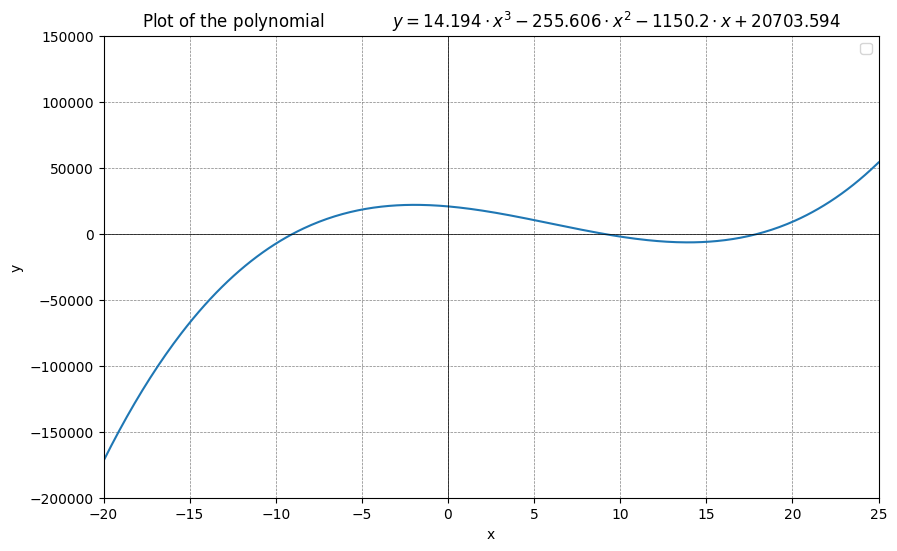
\includegraphics[width=14cm]{polynomial-plot}
\end{center}

\noindent С помощью библиотеки scipy найдем эталонные корни уравнения
\begin{equation*}
    [-9.000562591621339, \quad 8.997886402334267, \quad 18.010707751918982]
\end{equation*}
\begin{center}
    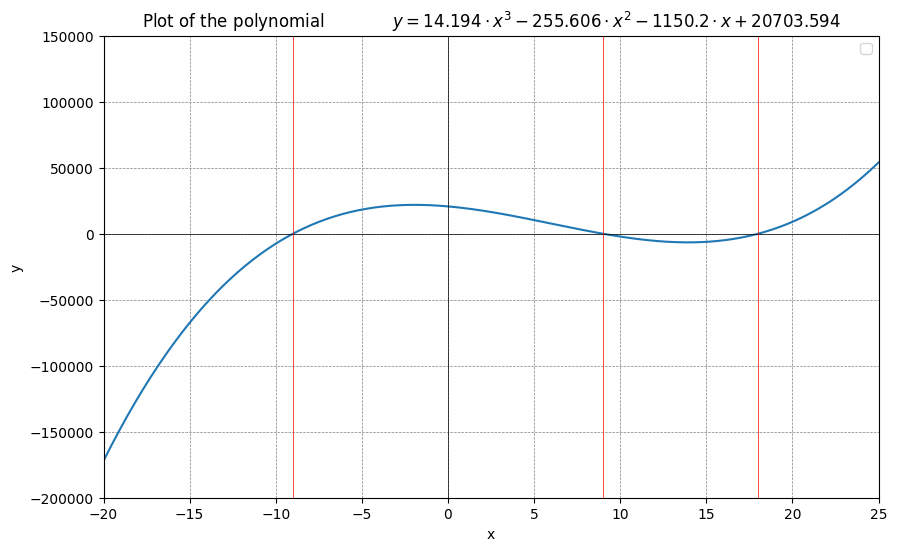
\includegraphics[width=14cm]{polynomial-plot-roots}
\end{center}

\noindent Найдем каждый из кореней тремя разными способами: 
\begin{itemize}
    \item Метод касательных (Ньютона).
    \item Метод секущих.
    \item Метод деления отрезка пополам.
\end{itemize}

\subsection*{Метод Ньютона}
Для нахождения левого корня уравнения воспользуемся методом касательных (Ньютона).\\
Рабочая формула
\begin{equation*}
    x_k = x_{k-1} - (f'(x_{k-1}))^{-1} \cdot f(x_{k-1})
\end{equation*}

\noindent Производную будем искать методом центральных разностей.\\
Рабочая формула
\begin{equation*}
    f'(x) \approx \cfrac{f(x + h) - f(x - h)}{2h}
\end{equation*}

\noindent В качестве $x_0$ возьмем -10.\\

\begin{align*}
    \begin{aligned}
        & k: 0 \\
        & x_{(0)}: -10 \\
        & x_{(1)}: -9.08164 \\
        & \\
    \end{aligned}
    \qquad
    \begin{aligned}
        & k: 1 \\
        & x_{(1)}: -9.08164 \\
        & x_{(2)}: -9.00116 \\
        & 0.08047849 > 0.0001
    \end{aligned}
    \qquad
    \begin{aligned}
        & k: 2 \\
        & x_{(2)}: -9.00116 \\
        & x_{(3)}: -9.00056 \\
        & 0.00060173 > 0.0001
    \end{aligned}
    \qquad
    \begin{aligned}
        & k: 3 \\
        & x_{(3)}: -9.00056 \\
        & x_{(4)}: -9.00056 \\
        & 3e-08 < 0.0001
    \end{aligned}
\end{align*}\\

\noindent Итого мы получили ответ с заданной погрешностью за k = 3 шагов

\subsection*{Метод деления отрезка пополам}
Для нахождения срединного корня уравнения воспользуемся методом деления отрезка пополам.\\
Данный метод может быть записан в виде псевдокода
\begin{tcolorbox}[colback=gray!10, colframe=gray!50, title=Псевдокод Метода Деления Отрезка Пополам]
    \begin{verbatim}
    input: Function f,
           endpoint values a, b,
           tolerance TOL,
           maximum iterations NMAX
    conditions: a < b,
                either f(a) < 0 and f(b) > 0 or f(a) > 0 and f(b) < 0
    output: value which differs from a root of f(x) = 0 by less than TOL
    
    N ← 1
    while N <= NMAX do // limit iterations to prevent infinite loop
        c ← (a + b)/2 // new midpoint
        if f(c) = 0 or (b – a)/2 < TOL then // solution found
            Output(c)
            Stop
        end if
        N ← N + 1 // increment step counter
        if sign(f(c)) = sign(f(a)) then a ← c else b ← c // new interval
    end while
    Output("Method failed.") // max number of steps exceeded
    \end{verbatim}
\end{tcolorbox}

\noindent В качестве отрезка [a, b] возьмем [5, 10].\\

\begin{align*}
    \begin{aligned}
        & k: 0 \\
        & a: 5 \\
        & b: 10 \\
        & c: 7.5 \\
        & f(c): 3687.35025 \\
        & 2.5 > 0.0001
    \end{aligned}
    \qquad
    \begin{aligned}
        & k: 1 \\
        & a: 7.5 \\
        & b: 10 \\
        & c: 8.75 \\
        & f(c): 578.38072 \\
        & 1.25 > 0.0001
    \end{aligned}
    \qquad
    \begin{aligned}
        & k: 2 \\
        & a: 8.75 \\
        & b: 10 \\
        & c: 9.375 \\
        & f(c): -849.40649 \\
        & 0.625 > 0.0001
    \end{aligned}
    \qquad
    \begin{aligned}
        & k: 3 \\
        & a: 8.75 \\
        & b: 9.375 \\
        & c: 9.0625 \\
        & f(c): -148.23685 \\
        & 0.3125 > 0.0001
    \end{aligned}
\end{align*}

\vspace{-5pt}

\begin{align*}
    \begin{aligned}
        & k: 4 \\
        & a: 8.75 \\
        & b: 9.0625 \\
        & c: 8.90625 \\
        & f(c): 212.05338 \\
        & 0.15625 > 0.0001
    \end{aligned}
    \qquad
    \begin{aligned}
        & k: 5 \\
        & a: 8.90625 \\
        & b: 9.0625 \\
        & c: 8.98438 \\
        & f(c): 31.13332 \\
        & 0.07812 > 0.0001
    \end{aligned}
    \qquad
    \begin{aligned}
        & k: 6 \\
        & a: 8.98438 \\
        & b: 9.0625 \\
        & c: 9.02344 \\
        & f(c): -58.74804 \\
        & 0.03906 > 0.0001
    \end{aligned}
    \qquad
    \begin{aligned}
        & k: 7 \\
        & a: 8.98438 \\
        & b: 9.02344 \\
        & c: 9.00391 \\
        & f(c): -13.85611 \\
        & 0.01953 > 0.0001
    \end{aligned}
\end{align*}

\vspace{-5pt}

\begin{align*}
    \begin{aligned}
        & k: 8 \\
        & a: 8.98438 \\
        & b: 9.00391 \\
        & c: 8.99414 \\
        & f(c): 8.62646 \\
        & 0.00977 > 0.0001
    \end{aligned}
    \qquad
    \begin{aligned}
        & k: 9 \\
        & a: 8.99414 \\
        & b: 9.00391 \\
        & c: 8.99902 \\
        & f(c): -2.61786 \\
        & 0.00488 > 0.0001
    \end{aligned}
    \qquad
    \begin{aligned}
        & k: 10 \\
        & a: 8.99414 \\
        & b: 8.99902 \\
        & c: 8.99658 \\
        & f(c): 3.00354 \\
        & 0.00244 > 0.0001
    \end{aligned}
    \qquad
    \begin{aligned}
        & k: 11 \\
        & a: 8.99658 \\
        & b: 8.99902 \\
        & c: 8.9978 \\
        & f(c): 0.19265 \\
        & 0.00122 > 0.0001
    \end{aligned}
\end{align*}

\vspace{-5pt}

\begin{align*}
    \begin{aligned}
        & k: 12 \\
        & a: 8.9978 \\
        & b: 8.99902 \\
        & c: 8.99841 \\
        & f(c): -1.21266 \\
        & 0.00061 > 0.0001
    \end{aligned}
    \qquad
    \begin{aligned}
        & k: 13 \\
        & a: 8.9978 \\
        & b: 8.99841 \\
        & c: 8.99811 \\
        & f(c): -0.51002 \\
        & 0.00031 > 0.0001
    \end{aligned}
    \qquad
    \begin{aligned}
        & k: 14 \\
        & a: 8.9978 \\
        & b: 8.99811 \\
        & c: 8.99796 \\
        & f(c): -0.15869 \\
        & 0.00015 > 0.0001
    \end{aligned}
    \qquad
    \begin{aligned}
        & k: 15 \\
        & a: 8.9978 \\
        & b: 8.99796 \\
        & c: 8.99788 \\
        & f(c): 0.01698 \\
        & 8e-05 < 0.0001
    \end{aligned}
\end{align*}\\

\noindent Итого мы получили ответ с заданной погрешностью за k = 15 шагов

\subsection*{Метод секущих}
Для нахождения правого корня уравнения воспользуемся методом секущих.\\
Рабочая формула
\begin{equation*}
    x_k = x_{k-1} - \cfrac{(b - x_{k-1})f(x_{k-1})}{f(b)-f(x_{k-1})}
\end{equation*}

\noindent В качестве отрезка [a, b] возьмем [15, 20];\\
\noindent В качестве $x_0$ возьмем 15.\\

\begin{align*}
    \begin{aligned}
        & k: 0 \\
        & x_{(0)}: 15 \\
        & x_{(1)}: 17.02965 \\
        & \\
    \end{aligned}
    \qquad
    \begin{aligned}
        & k: 1 \\
        & x_{(1)}: 17.02965 \\
        & x_{(2)}: 17.75509 \\
        & 0.72544 > 0.0001
    \end{aligned}
    \qquad
    \begin{aligned}
        & k: 2 \\
        & x_{(2)}: 17.75509 \\
        & x_{(3)}: 17.94866 \\
        & 0.19357 > 0.0001
    \end{aligned}
\end{align*}

\vspace{-5pt}

\begin{align*}
    \begin{aligned}
        & k: 3 \\
        & x_{(3)}: 17.94866 \\
        & x_{(4)}: 17.99592 \\
        & 0.04726 > 0.0001
    \end{aligned}
    \quad
    \begin{aligned}
        & k: 4 \\
        & x_{(4)}: 17.99592 \\
        & x_{(5)}: 18.0072 \\
        & 0.01128 > 0.0001
    \end{aligned}
    \qquad
    \begin{aligned}
        & k: 5 \\
        & x_{(5)}: 18.0072 \\
        & x_{(6)}: 18.00988 \\
        & 0.00268 > 0.0001
    \end{aligned}
\end{align*}

\vspace{-5pt}

\begin{align*}
    \begin{aligned}
        & k: 6 \\
        & x_{(6)}: 18.00988 \\
        & x_{(7)}: 18.01051 \\
        & 0.00063 > 0.0001
    \end{aligned}
    \qquad
    \begin{aligned}
        & k: 7 \\
        & x_{(7)}: 18.01051 \\
        & x_{(8)}: 18.01066 \\
        & 0.00015 > 0.0001
    \end{aligned}
    \qquad
    \begin{aligned}
        & k: 8 \\
        & x_{(8)}: 18.01066 \\
        & x_{(9)}: 18.0107 \\
        & 4e-05 < 0.0001
    \end{aligned}
\end{align*}\\

\noindent Итого мы получили ответ с заданной погрешностью за k = 8 шагов

\subsection*{Вывод}

\begin{center}
    \begin{tikzpicture}[scale = 0.4]
        % box 2
        \draw[line width=2pt, rounded corners=5pt] (0,0) rectangle (6,7);
    
        % number 2
        \node at (3,3.5) {\fontsize{20}{24}\selectfont\bfseries 2};
    
        % text 2
        \node at (3,9) {Метод};
        \node at (3,8) {секущих};

        % box 1
        \draw[line width=2pt, rounded corners=5pt] (6.5,0) rectangle (12.5,13);
    
        % number 1
        \node at (9.5,6.5) {\fontsize{20}{24}\selectfont\bfseries 1};
    
        % text 1
        \node at (9.5,15) {Метод};
        \node at (9.5,14) {Ньютона};

        % box 3
        \draw[line width=2pt, rounded corners=5pt] (13, 0) rectangle (19, 4);
    
        % number 3
        \node at (16, 2) {\fontsize{20}{24}\selectfont\bfseries 3};

        % text 3
        \node at (16,8) {Метод};
        \node at (16,7) {деления};
        \node at (16,6) {отрезка};
        \node at (16,5) {пополам};
    \end{tikzpicture}
\end{center}

\end{document}
